
\documentclass{gji}
\usepackage{timet,color}
\usepackage[urlcolor=blue,citecolor=black,linkcolor=black]{hyperref}
\usepackage{graphicx}
\begin{document}
\tableofcontents
\newpage

\title{Novel methodology for virtual machine introspection}

\section{Results and discussion }
This research developed the AGM-AB model that is implemented using the Python tool and for estimating the effectiveness of the introduced model, several metrics like accuracy, precision, FPR value, recall, F-measure, and AUC are calculated.

\subsection{Case study}
In this research, the novel deep learning approach is developed for increasing the security of VMs in the cloud service. Let 10 numbers of virtual machines in cloud service for analyzing the security. 
$$
F1 - score= 2 \int \frac{P*R}{P+R}dP
$$
The F1-measure value of the introduced AGM-AB manner has been evaluated by prevailing methods like AMMD, IMI, TKRD, RF, AMD, and Ensemble learning.
\par The feature selection process is utilized to enhance the classification of benign and malware executable. Hence, the proposed model has effectively detected the normal executable files and malware. Malware classification using the proposed AGM-AB model is represented in Figure ~\ref{Figure 1:image}.
\begin{figure}
  \centering
  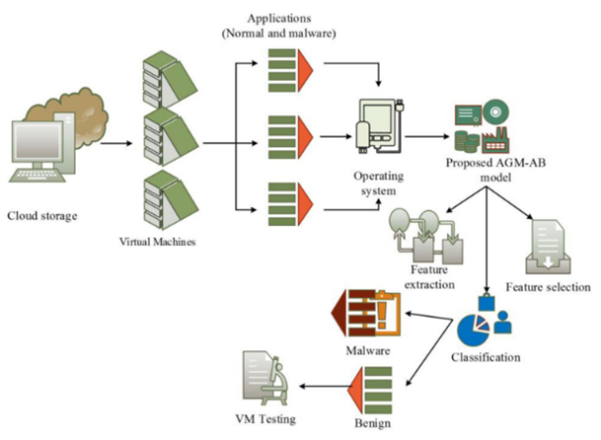
\includegraphics[width=0.8\linewidth]{Figures/fig1.png}
  \caption{Malware classification in VM}
  \label{Figure 1:image}
\end{figure}

\subsection{Related works}
Several existing techniques are reviewed above, from that some issues in VMI such as network error, malicious attacks, VMI security, high computation time and high FPR rate were recognized. These issues have been motivated this research to enhance the performance of detecting malware, True Positive Rate (TPR), False Prediction Rate (FPR), error rate and so on. The key contributions of this research work involves,

\begin{enumerate}
\item Initially, the collected dataset is trained to the system that involves malware and benign files;
\item Moreover, a novel AGM-AB algorithm is developed for detecting unknown malware functions from the benign program;
\item Additionally, the African buffalo fitness module has been updated in the AGM manner to extract the features of the Virtual Machine Monitor (VMM);
\item Here, the introduced AGM-AB model investigates the guest operating system, system calls, and kernel data for classifying the malware and benign files;
\item Also, the AGM-AB approach is tested by launching faults and malware functions to demonstrate the effectiveness of the AGM-AB method;
\item Subsequently, the implementation of this proposed AGM-AB approach is done in the Python tool and the metrics are computed;
\item Finally, the proposed method is evaluated by prevailing approaches in terms of recall, accuracy, AUC, FPR, precision, and F-measure;
\end{enumerate}

\subsection{Design of the Method}
This section details the design and operation of the proposed method to analyze malware in a Virtual Machine through Virtual Machine Introspection technique. It consists of the following five steps: 
\begin{enumerate} 
  \item Access to the asset: This is achieved through the interprocess mechanism called COM/XPCOM that implements the VirtualBox API;
  \item Collection: It generates a memory dump of the Virtual Machine volatile memory;
  \item Analysis: It translates the low-level bytes into high-level information with the help of the Volatility tool, through the profile of the virtual machine and extracts objects from the operating system;
  \item Logging: It generates the log of the malware analysis;
  \item Containment: The COM/XPCOM interprocess mechanism sends a killing command to finish the malware execution from outside the Virtual Machine;
\end{enumerate}
\section {Performance metrics}
FN characterizes the false-negative rate for evaluating the inaccurate detection of the malware files and FP denotes the false-positive value for calculating the inaccurate detection of benign files (Table ~\ref{tab:freq1}).
\begin{table}
  \caption{Summary of state-of-the-art approaches}
  \label{tab:freq1}
  \begin{tabular}{cc}
    Author&Methods\\
        Mishra et al.&KVM Inspector and ML\\
        Kumara and Jaidhar&ML, RF MFA, and leveraging VMI\\
        Patil et al.&AMD\\
        Zhang et al.&Detection model using MFA\\
        Kumara and Jaidhar&AMMDS\\
        Kordestani et al.&LSS\\
        Kordestani and Saif&observer-based mitigation and attack detection framework\\
        Kiperberg&Virtualization based method\\
        Proposed&AGM-AB\\
\end{tabular}
\end{table}
\par Initially, the dataset is collected from a GitHub source that is named as ‘ember’ for performing the process that involves malware and benign files. Initially, the dataset Ds is trained to the system using Eq:
$$
D_s =  \{\ x_n y_n\}\ ; \{\ n = 1,2,3...\}\,
$$
\par Where, $x_n$ is represents the benign executable files, $y_n$ represents the malware files in the virtual machine
\par It is calculated by the number of incorrect and correct predictions which is summarized by count values. It is used to summarize the performance of classified malware files on the position of tested and trained data. Additionally, the confusion matrix is represented in Figure ~\ref{Figure 2:image}, where, TP denotes the true positive for calculating the accurate detection of the malware files in the dataset. 
\begin{figure}
  \centering
  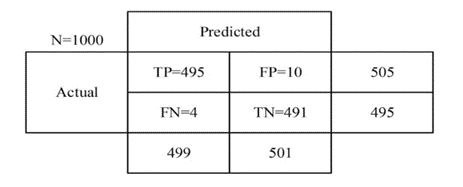
\includegraphics[width=0.8\linewidth]{Figures/fig2.png}
  \caption{Confusion matrix}
  \label{Figure 2:image}
\end{figure}

\subsection{False positive rate (FPR)}
\par FPR denotes the false-positive ratio that is defined as the ratio between inaccurately detected benign files and the total quantity of FP and TN values, which is calculated using Eq (~\ref{eq1:equation}),
\begin{equation}
A = \frac{\frac{TP+TN}{FPR+FN}}{TN+FP+TP+FN}
\label{eq1:equation}
\end{equation}
\par The FPR rate of the introduced AGM-AB approach is evaluated by prevailing methods like RF, AMD, TKRD, IMI, AMMD and Ensemble learning approaches, which are detailed in Table ~\ref{tab:freq2}.
\begin{table}
  \caption{Comparison of FPR}
  \label{tab:freq2}
  \begin{tabular}{cccccccc}
    Number of executable files in VM&RF&AMD&Ensemble learning&TKRD&AMMD&IMI&AGM-AB\\
       100& 0.004	&3.70	&0.322&	0.603&	0.005&	0.13&	0.001\\
       200&	0.006&	3.72	&0.43	&0.71&0.009	&0.22&	0.002.\\
        300&	0.027&	3.85&	0.58	&0.88	&0.0016&	0.37	&0.0035\\
       400&	0.093&	3.95&	0.67&	1.02&	0.0023&	0.47&	0.004\\
       500&	0.075&	4.37&	1.04&	1.10&	0.0034&	0.53&	0.005\\
\end{tabular}
\end{table}
The inaccurate detection of the executable files should be less for an efficient approach.
\end{document}